\section{Subsystem Decomposition}
The \texttt{DriveIT System} can be split into five main subsystems - the \texttt{DriveIT Windows Client}, \texttt{CarQuery}, \texttt{DriveIT Web Client}, \texttt{DriveIT Web API}, and \texttt{Persistent Storage} subsystems. 
These subsystems are described below. 

\subsection{The DriveIT System}
\begin{figure}[H]
	\centering
	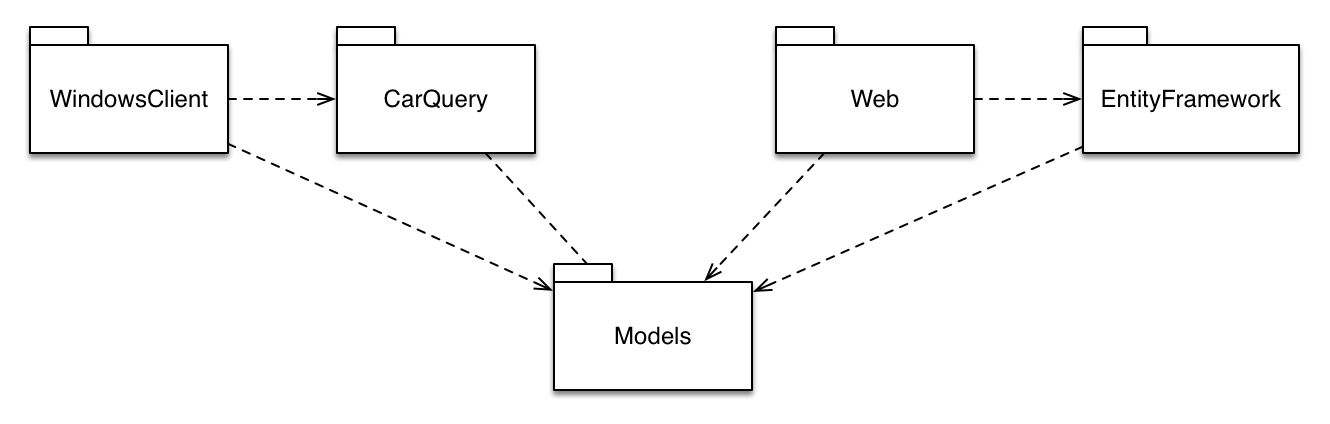
\includegraphics[width=\textwidth]{Figures/DriveITSubsystemDecomposition}\\
	\caption{Subsystems of the \texttt{DriveIT System}.}
\end{figure}

\subsection{Persistent Storage Subsystem} 
The Persistent Storage Subsystem manages storing and retrieving entity objects using the \textit{Entity Framework} and its serialisation functionality.\\
The serialised entities are stored in a \textit{Microsoft SQL Database} which is hosted on \textit{Microsoft Azure}. The subsystem provides the \texttt{DriveIT Web API} with deserialised entities, which uses the entities to provide the backend for other subsystems.\\
The subsystem supports retrieving all Entities of a given type, a specific entity using its unique ID, and retrieving an entity on its relation to other entities.
The Persistent Storage Subsystem consists of two classes and an interface (see figure \ref{fig:entityframeworksubsystem}). \texttt{EntityStorage} is the repository working on top of the \textit{Entity Framework} database layer, \texttt{DriveITContext}, providing the \texttt{IPersistentStorage} interface.

\begin{figure}[H]
	\centering
	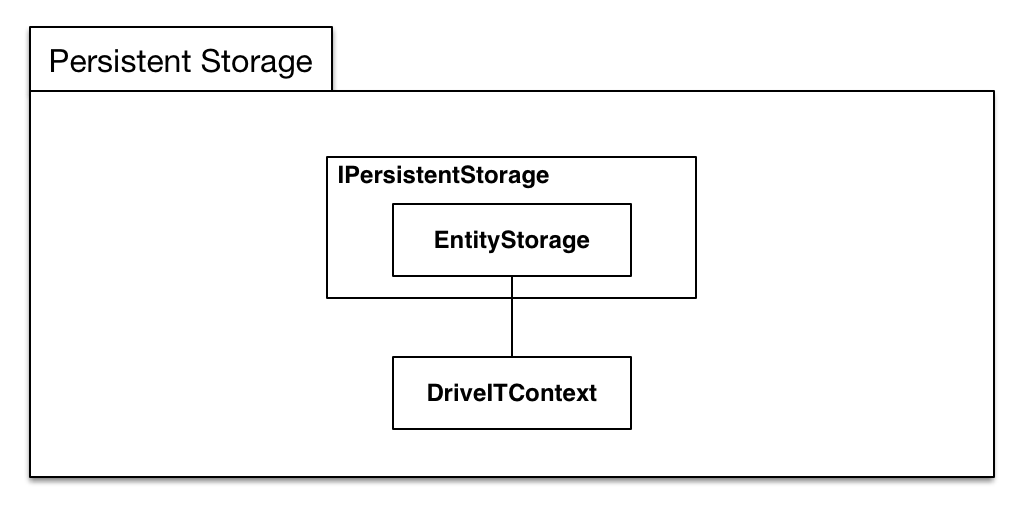
\includegraphics[width=\textwidth]{Figures/EntityFrameworkSubsystemDecomposition}
	\caption{Classes in the Persistent Storage Subsystem.}
	\label{fig:entityframeworksubsystem}
\end{figure}

\subsection{Web API}
The \texttt{DriveIT Web API}, which is built on \textit{ASP.NET Web API}\footnote{\url{http://www.asp.net/web-api}}, provides public communication with the \texttt{Persistent Storage} subsystem. This is done using specific URL routes. Furthermore it enforces authorisation so unauthorized users, and users with different user roles, only have limited access to the data of the \texttt{DriveIT System}.\\ 
Every table in the \texttt{Persistent Storage} subsystem must therefore be supported by the web API, although not every table is available to every user.\\
The \texttt{DriveIT Web API} is comprised of a series of modules for serialising the Model Entities into \texttt{JSON}\footnote{\url{http://en.wikipedia.org/wiki/JSON}} or \texttt{XML}\footnote{\url{http://en.wikipedia.org/wiki/XML}} and transferring these via a \texttt{REST} interface accessible using \texttt{HTTP}.\\
These modules are built into \textit{ASP.NET Web API}, and are not handled in our code.\\

The Web API consists of several controllers which uses a static class to translate \texttt{DTO's}\footnote{\url{http://en.wikipedia.org/wiki/Data_transfer_object}} into entities and vice versa. It is also the controllers that check for special cases, e.g. when a customer wants to update or delete a comment, and it is not allowed to change other \texttt{Customer}s' comments.

\subsection{Windows Client} 
\begin{figure}[H]
	\centering
	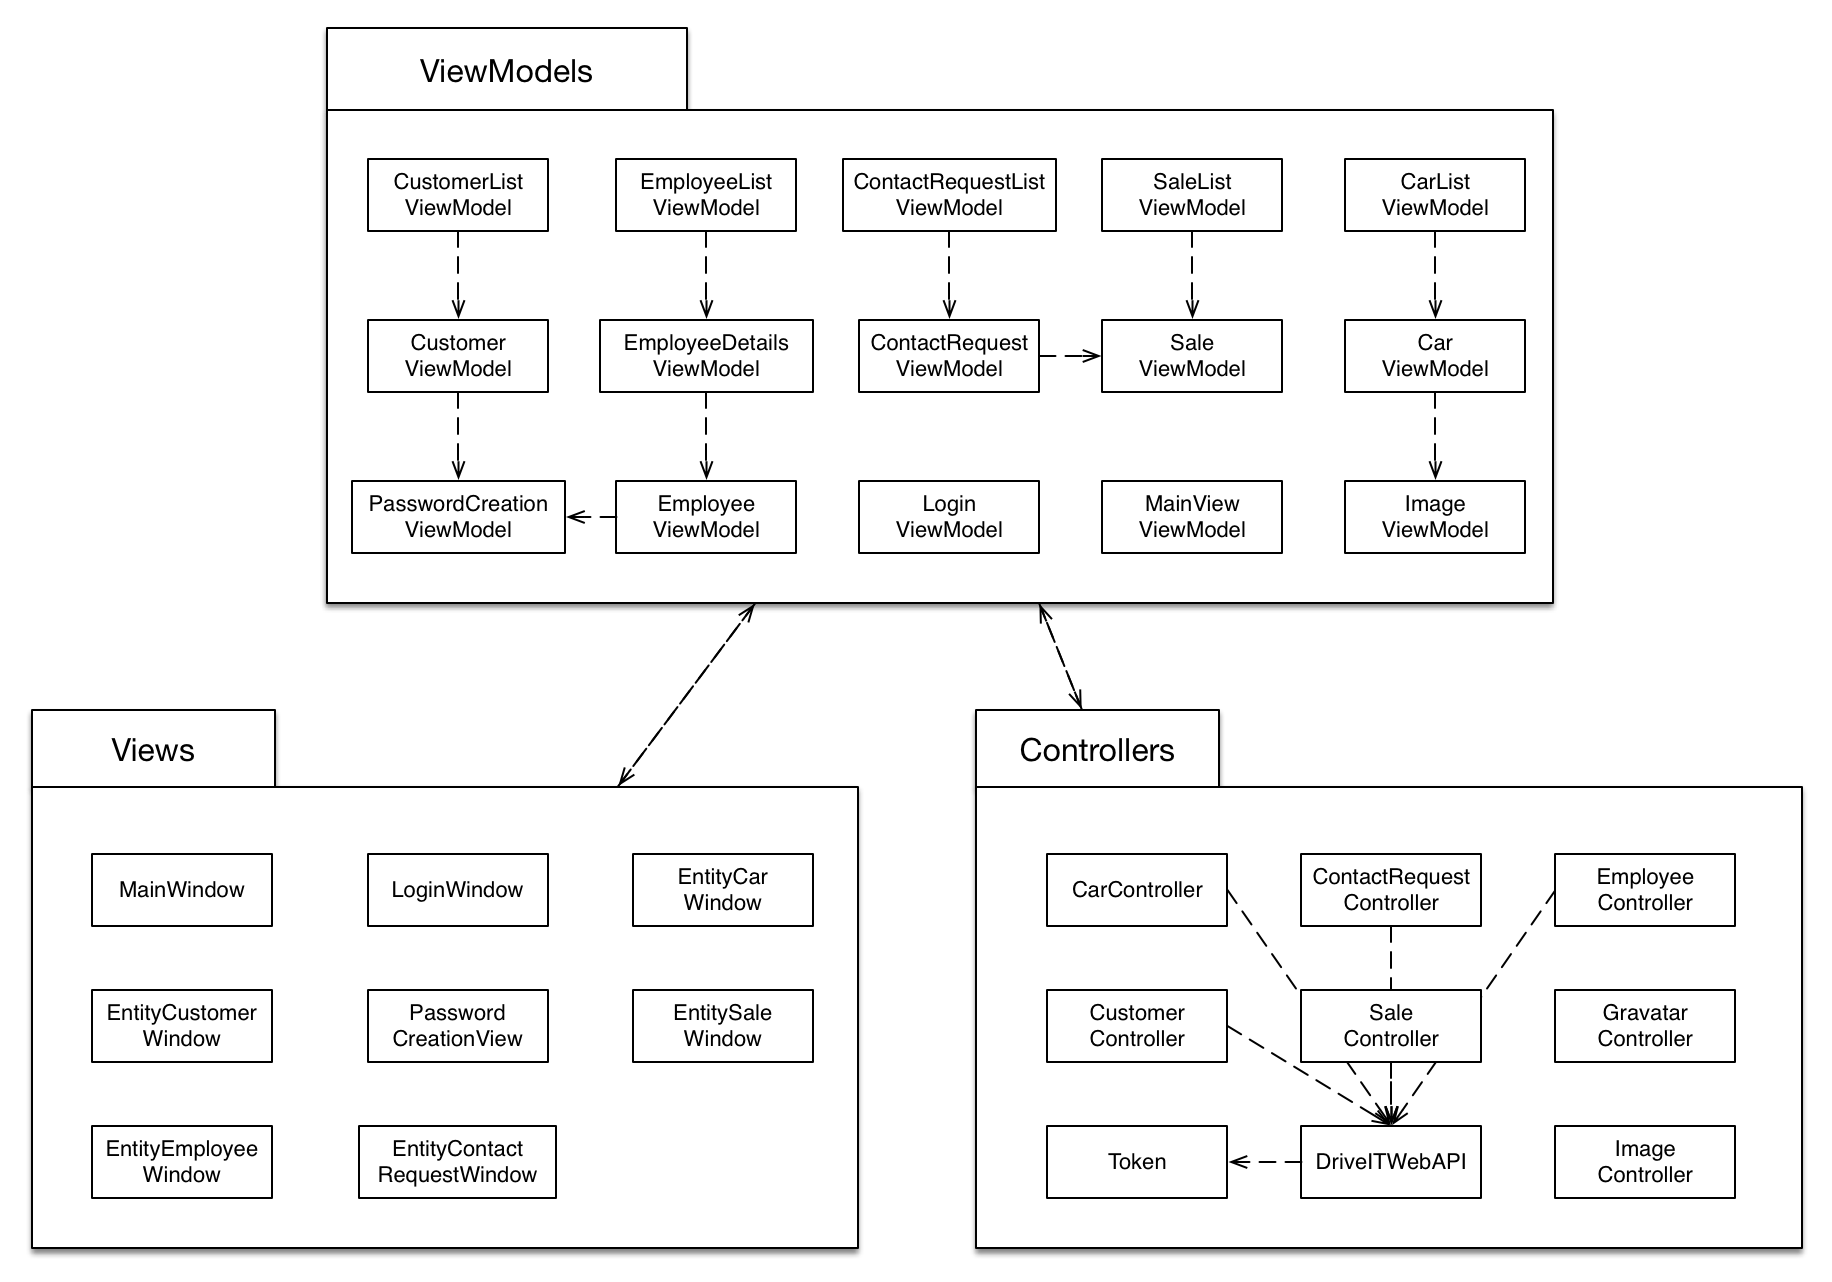
\includegraphics[width=\textwidth]{Figures/WindowsClientCodeMapProper}
	\caption{The Code Map of the Windows Client}
	\label{fig:WindowsClientCodeMap}
\end{figure}
The \texttt{DriveIT Windows Client} is used by the \texttt{Employee}s, to manipulate data in the \texttt{DriveIT System}. Depending on their role, \texttt{Employee} or \texttt{Administrator}, they can \textit{CRUD} all entities except for creating \texttt{ContactRequest}s.\\

The \texttt{Employee} signs in to the client with his or her email and password, and can then use the user interface to manipulate data in the \texttt{DriveIT System}.

The subsystem is made out of three main components: The \texttt{Views}, the \texttt{ViewModels} and the \texttt{Controllers}.

The \texttt{Views} package contains the user interface written in Windows Presentation Foundation (henceforth WPF). The \texttt{ViewModels} package contains the \texttt{ViewModel}s which hold data bound to the \texttt{View}s following Microsoft's \textit{Model View ViewModel} architectural pattern\footnote{\url{http://en.wikipedia.org/wiki/Model_View_ViewModel}}.

\texttt{ViewModel}s for entities are often created in the form of a \texttt{EntityListViewModel} and a \texttt{EntityViewModel}, but a few extra \texttt{ViewModel}s exists for additional \texttt{View}s such as the \texttt{LoginViewModel} and the \texttt{PasswordCreationViewModel}.

The \texttt{Controllers} package contains the \texttt{Controller}s which transforms data and sends and receives HTTP requests to and from the \texttt{DriveIT Web API}. Images are uploaded to \textit{Azure Blob Storage}. To provide \texttt{Employee}s and \texttt{Customer}s with profile pictures, a \texttt{GravatarController} exists to convert email strings into \textit{Gravatar} profile URLs.

\subsection{Web Client}
The \texttt{DriveIT Web Client} is accessible through the Internet, where it is being used by non-registered and registered \texttt{Customer}s. The \texttt{DriveIT Web Client} is being used to search for \texttt{Car}s, that are up for sale in the \texttt{DriveIT System}.

The \texttt{DriveIT Web Client} allows the \texttt{Customer} to \textit{CRUD} \texttt{Comment}s if signed in. Otherwise \texttt{Comment}s can only be read.

It is also possible to \textit{create}, \textit{read} and \textit{delete} \texttt{ContactRequest}s and to read \texttt{Order}s and \texttt{Employee}s. A \texttt{Customer} is also able to \textit{read} and \textit{update} information regarding their own account.

It is possible to create an account on the web page with a non registered email.

The \texttt{DriveIT Web Client} is based on the \textit{ASP.NET MVC} framework\footnote{\url{http://www.asp.net/mvc}}, that is implementing the \textit{Model View Controller} design pattern (see section \ref{sec:MVC}).

The \textit{MVC} subsystem would usually consist of three components: Models, Views and Controllers. However, since the \texttt{DriveIt Web Client} directly references the controllers from the \texttt{DriveIT Web API}, the \texttt{MVC} subsystem uses the same models as the \texttt{Web API}. A regular \textit{ASP.NET MVC} project, would have its own models for persistence. The \textit{MvcControllers} create instances of the corresponding \textit{ApiControllers} and use these to retrieve the objects from the \texttt{DriveIT.Models} and serve them to the \textit{Views} as \textit{Models}. These \textit{Models} are then used in the views to represent the different DTO's.

\subsection{CarQuery} 
This subsystem is a collection of classes that enable the the \texttt{DriveIT Windows Client} to fill out missing information about cars, using the \textit{CarQuery API}.\\
The subsystem is used by an \texttt{Employee} when creating or updating a \texttt{Car}. The subsystem consists of a \textit{JSON} deserialiser that communicates with the \textit{CarQuery API} and another class that receives a \texttt{Car} object and fills out the missing attributes using the deserialised \textit{JSON} data.

An \texttt{Employee} fills out the known information about the \texttt{Car} and the \texttt{CarQuery} subsystem then creates its query on the \textit{CarQuery API}.

Only the \texttt{CarQuery} static class is publicly accessible. As seen in figure \ref{fig:carquerysubsystem} it uses a \texttt{JSONWrapper} to receive data from the \textit{CarQuery API} and deserialises it into a \texttt{Trims} object which is an array of \texttt{Trim} objects holding the actual \texttt{Car} data.
\begin{figure}[H]
	\centering
	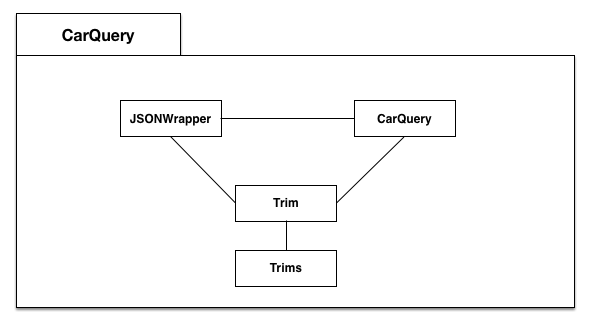
\includegraphics[width=\textwidth]{Figures/CarQuerySubsystemDecomposition}\\
	\caption{Classes of the \texttt{CarQuery} Subsystem.}
	\label{fig:carquerysubsystem}
\end{figure}
